% preamble with all definitions
\documentclass[12pt,letterpaper]{article}
\usepackage[utf8]{inputenc}
\usepackage[english]{babel}
\usepackage{amsmath}
\usepackage{amsfonts}
\usepackage{amssymb}
\usepackage{graphicx}
\usepackage{multirow}
\usepackage{fancyvrb}
\usepackage[breaklinks=true]{hyperref}
\usepackage[hyphenbreaks]{breakurl}
\hypersetup{
       pdfauthor = {Kim Siang Khaw},
        colorlinks=true, citecolor=blue, linkcolor=blue, bookmarksnumbered = true,
}
\usepackage[left=2cm,right=2cm,top=2cm,bottom=2cm]{geometry}

%%%%%%%Some style changes
\usepackage{caption}
\setlength{\captionmargin}{10mm}
\renewcommand\captionfont{\it}
\renewcommand\captionlabelfont{\bf}


\author{Wes Gohn, Tim Gorringe, Ran Hong, Kim Siang Khaw\thanks{Corresponding author, khaw84@uw.edu}, David Sweigart}
\title{\textbf{DAQ data structure for the Muon g-2 experiment}}
\begin{document}
\newcolumntype{C}[1]{>{\centering\arraybackslash}p{#1}}

\maketitle

\abstract{
This document outlines the DAQ data structure of the Muon g-2 experiment.
A detailed list of the MIDAS data bank will be shown and their contents will 
described.}

\tableofcontents
\newpage

\section{Introduction}

\subsection{Data unpacking in a nutshell}

The basic idea of data unpacking is to convert compact DAQ information stored in MIDAS banks to well-structured data products, as depicted in Fig.~\ref{fig:DataUnpacking}. Several unpackers are used to decode the information stored in MIDAS banks and the outputs are stored in different data products which are basically structs in C++ language.
A compact list of the Midas bank - Data unpacker - Data product is summarized in Sec.~\ref{sec:cheatsheet}.

\begin{figure}[htbp]
\centering
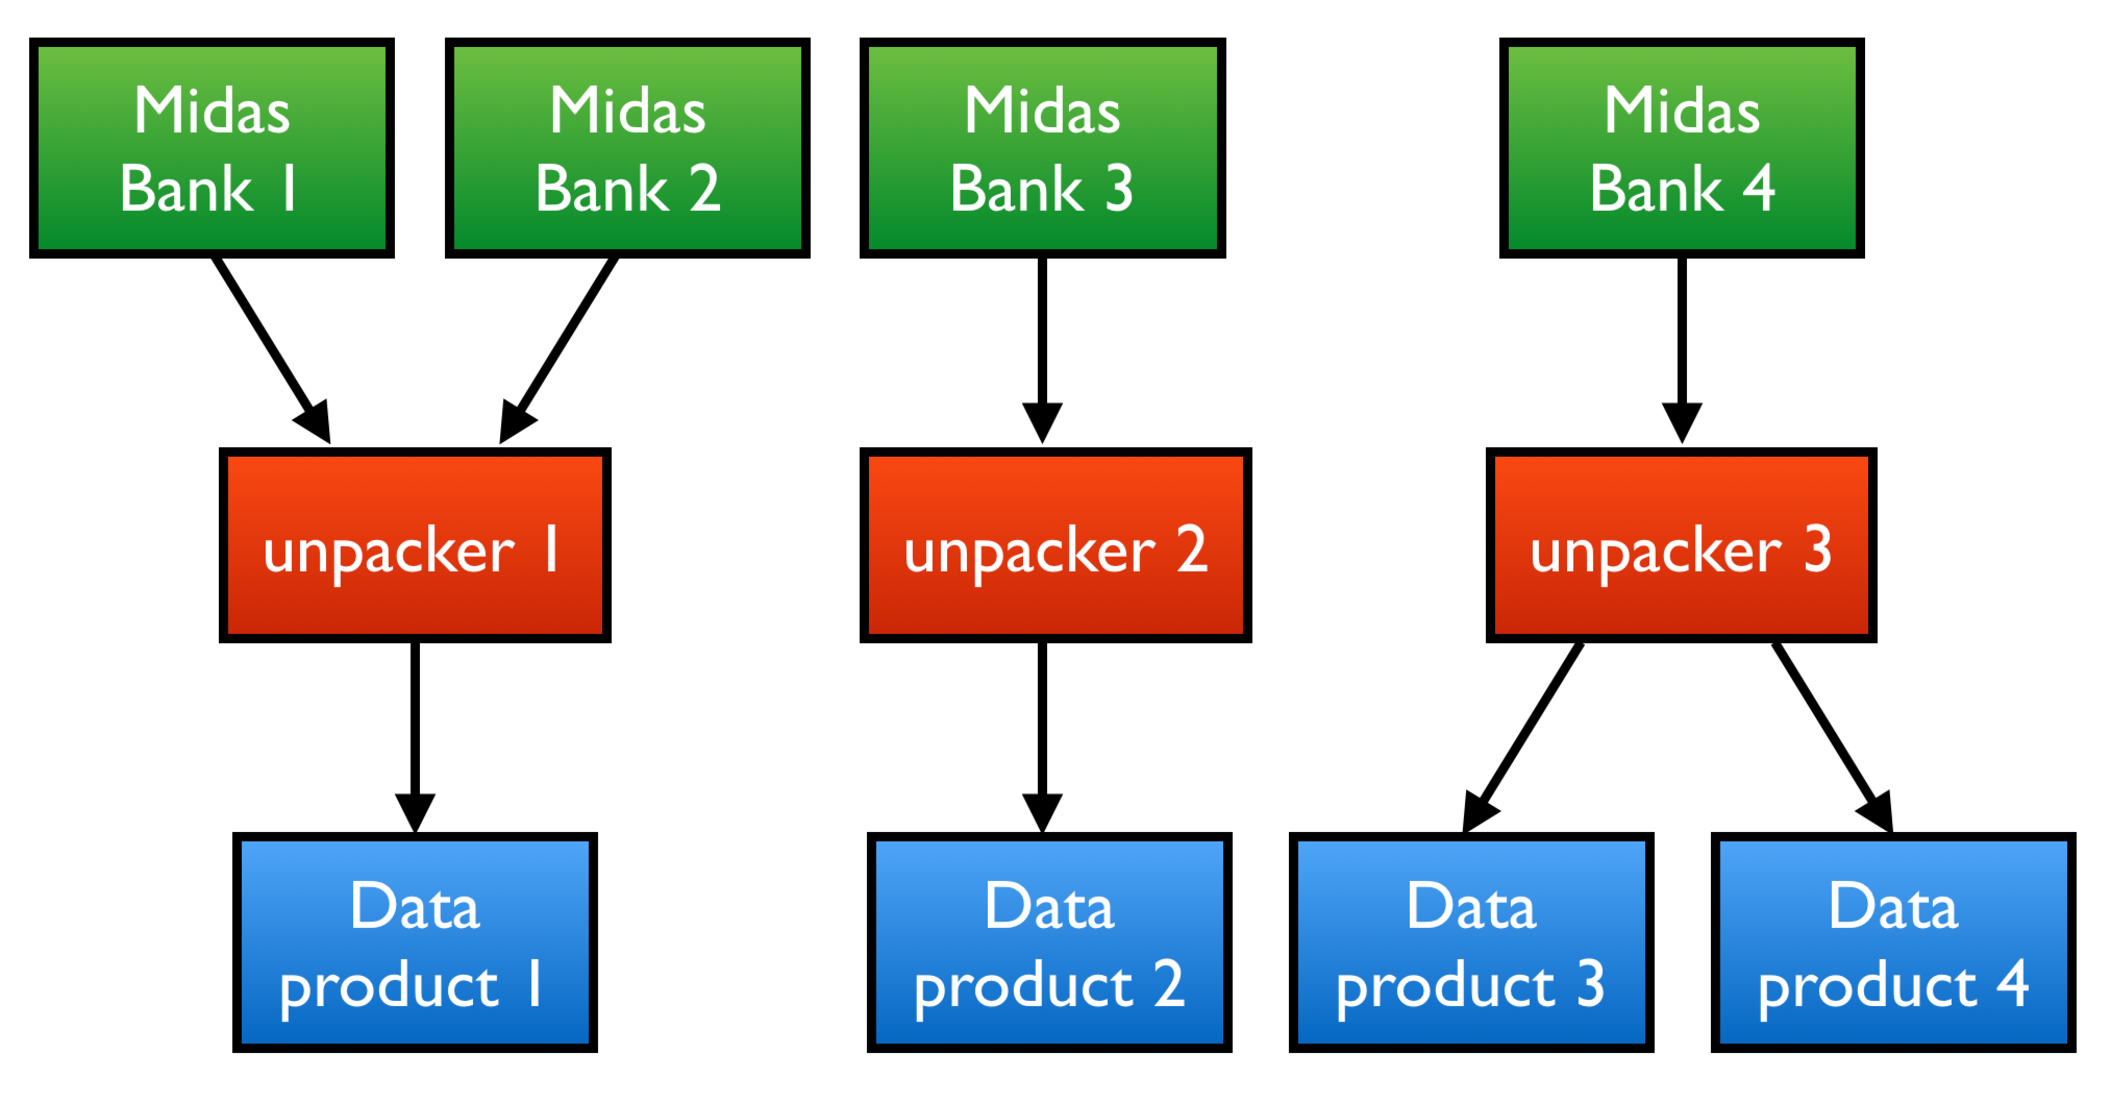
\includegraphics[width=0.65\textwidth]{pics/DataUnpacking.pdf} 
\caption{Simplified diagram of the flow of the data unpacking.}\label{fig:DataUnpacking}
\end{figure}


\subsection{MIDAS DAQ output in a nutshell}
The main DAQ framework for the Muon g-2 experiment is based on MIDAS~\cite{Midas}. 
MIDAS event structure is as depicted in Fig.~\ref{fig:MIDASEventStructure}.

\begin{figure}[htbp]
\centering
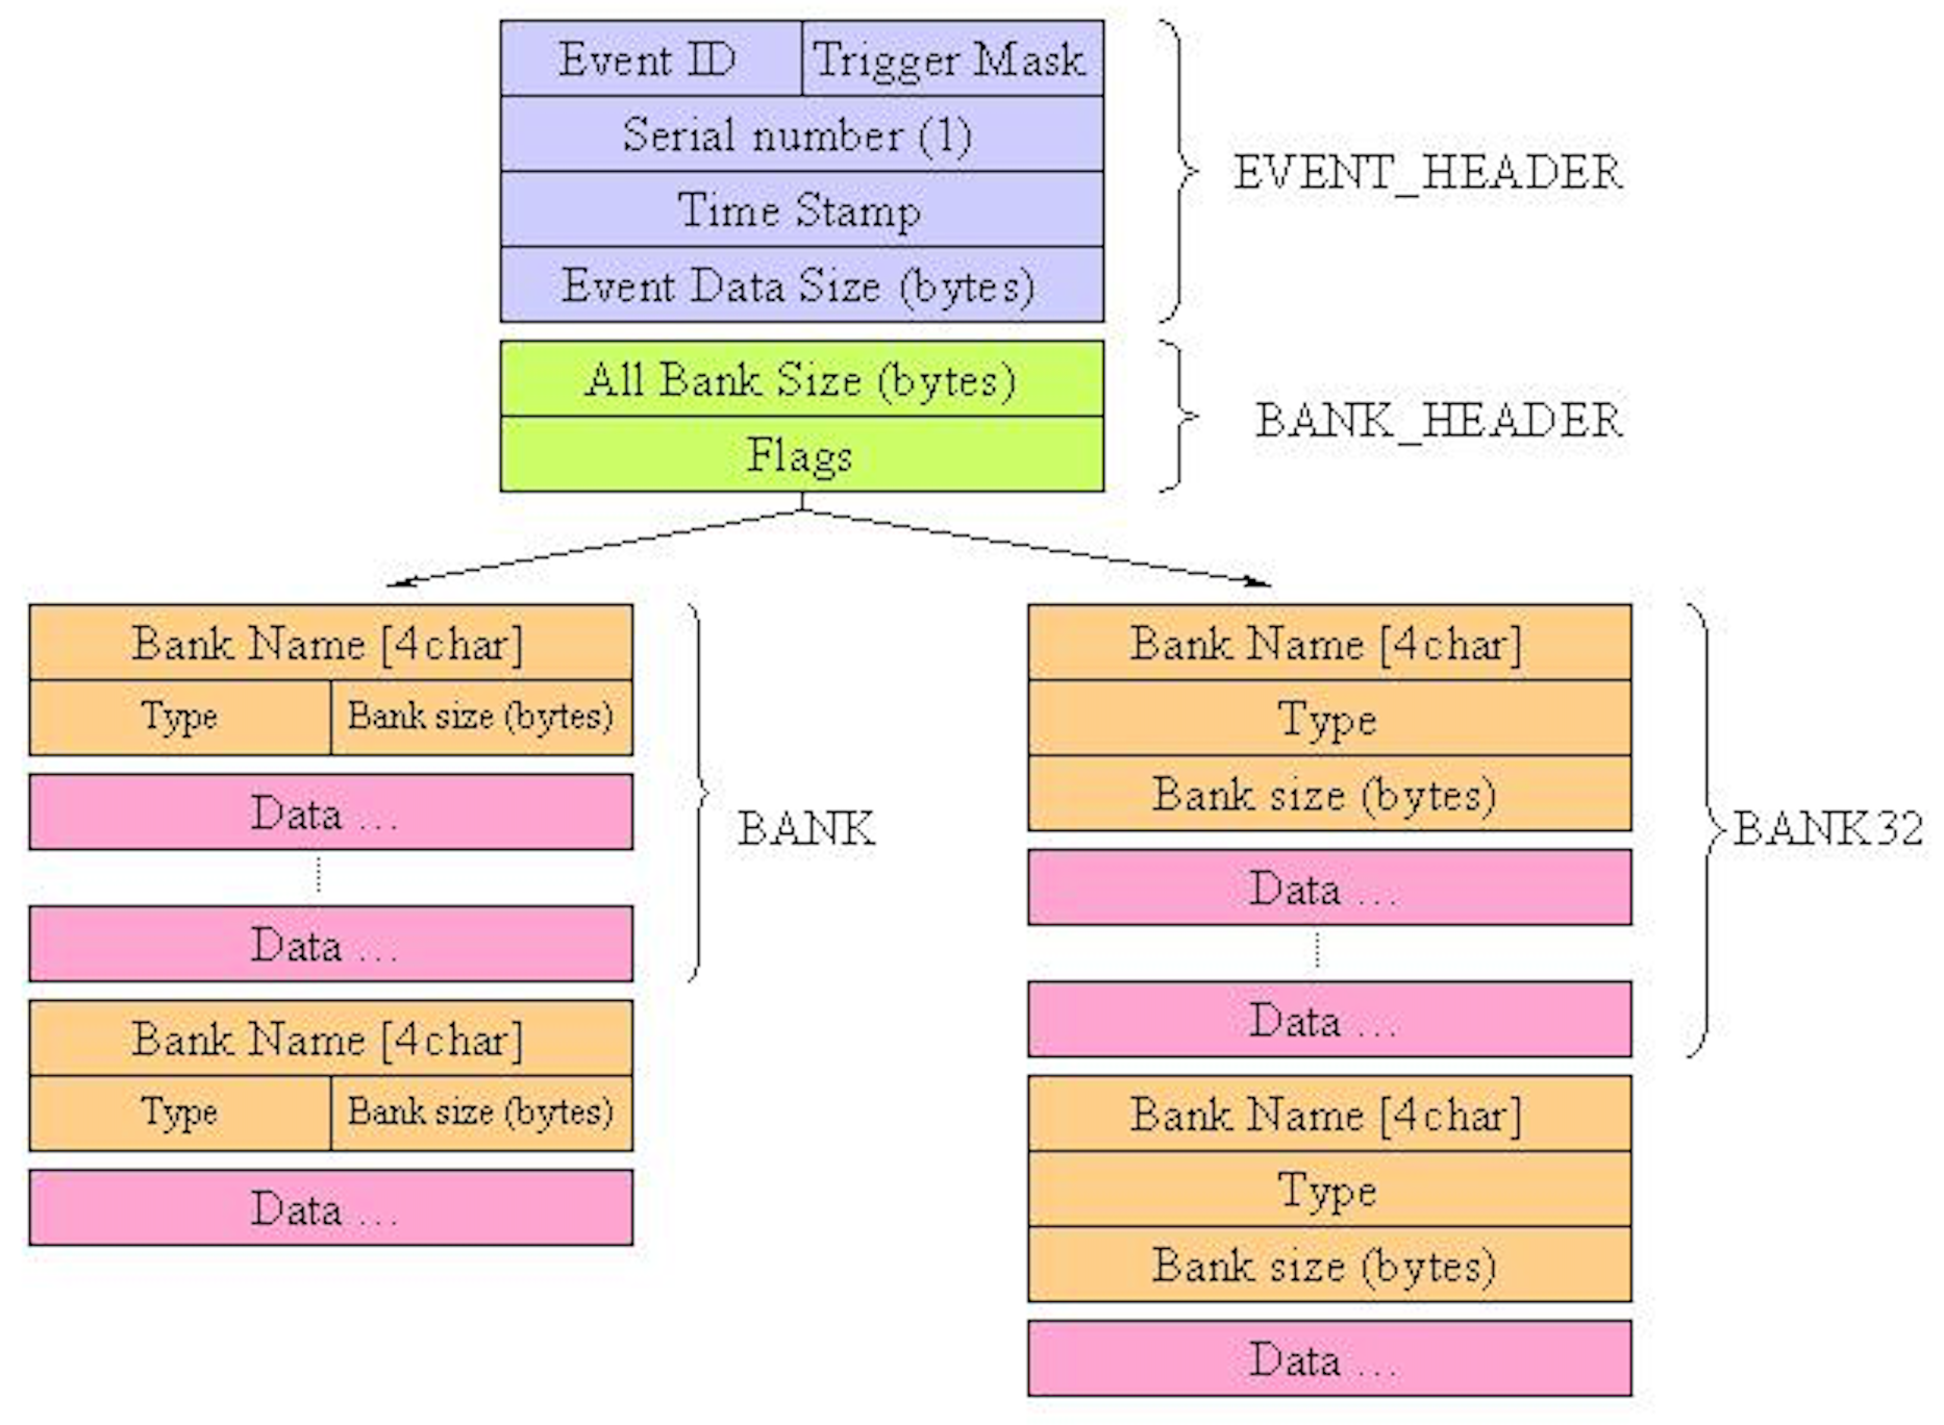
\includegraphics[width=0.6\textwidth]{pics/MIDASEventStructure.pdf} 
\caption{MIDAS event structure. Each event has its header that is followed by the bank header. Then all the banks will appear according the defined order.}\label{fig:MIDASEventStructure}
\end{figure}

\section{MIDAS Bank list}

Hundred of banks will be stored in each MIDAS event and it is very important to classify them properly. At the moment they can be grouped into 4 categories: calorimeter, auxiliary detector, CCC and magnetic field. Naming of these banks will be described in this section and their contents will be explained in the next section.

\subsection{Calorimeter-related banks}

There are 3 fill types for the calorimeter. \verb+Muon+ fill is the typical muon events, laser fill is event dedicated for laser calibration and monitoring events and pedestal fill is trivia from its name. Data from each fill type is identified from the bank name. The muon fill is denoted by ``\textbf{C}", the laser fill is denoted by ``\textbf{L}" and the pedestal fill is denoted by ``\textbf{P}". A summary of the banks is listed in Tab. \ref{tab:calotable}.

\begin{table}[htbp]
\centering
\caption{MIDAS bank list for the calorimetry data.}
\begin{tabular}{|c|c|c|C{8cm}|}
\hline 
muon fill& laser fill & pedestal fill  & \multirow{2}{*}{Description} \\ \cline{1-3}
\multicolumn{3}{|c|}{Bank name} & \\
\hline
CA & LA & PA & AMC13 Header \\ 
\hline 
CB & LB & PB & WFD5 header \\ 
\hline 
CC & LC & PC & GPU timing data \\ 
\hline 
CF & LF & PF & GPU fitted data \\ 
\hline 
CH & LH & PH & per-crystal Q-method data (N-th event, end of run) \\ 
\hline 
CL & LL & PL & Clock data \\ 
\hline 
CP & LP & PP & Pedestal\\ 
\hline 
CQ & LQ & PQ & per-calo Q-method data (every event) \\ 
\hline 
CR & LR & PR & WFD5 raw data \\ 
\hline 
CT & LT & PT & T-method islands \\ 
\hline 
CZ & LZ & PZ & AMC13 CDF trailers \\ 
\hline 
\end{tabular} 
\label{tab:calotable}
\end{table}

Since each bank has to be named exactly four characters, the last 2 characters denoted the calorimeter number, e.g. \textbf{CT03} means the T-method bank from calorimeter number 3.
Hence the number 01-24 are reserved for the calorimeters and 25 is reserved for the laser system.

\subsection{Auxiliary detector-related banks}

Systems that fall into the auxiliary detector category are the kickers, quadrupoles, IBMS, T0 counter and fiber harps. Depending on the length of the signal, two different types of digitizers will be used to digitize these signals: Cornell WFD5 and CANE 1742 digitizers. 
A separate T/Q-method is needed for auxiliary detectors. Their data banks are denoted with the initial ``\textbf{K}". A list of these banks are summarized in Tab. \ref{tab:auxtable}. The last 2 characters of the bank name will be decided soon.


\begin{table}[htbp]
\centering
\caption{MIDAS bank list for auxiliary T/Q data. This is mainly for the fiber harps, quads, kickers and IBMS.}
\begin{tabular}{|c|C{8cm}|}
\hline 
Bank name  & Description \\
\hline
KH &  Per aux. detector channel Q-method data (N-th event, end of run)\\
\hline
KQ &  Per aux. detector Q-method data (every event)\\
\hline
KT & T-method data \\
\hline
IBMS & IBMS waveforms \\
\hline
\end{tabular} 
\label{tab:auxtable}
\end{table}

\subsection{CCC related banks}

This is the bank storing the information regarding the CCC system based on FC7.
A list of these banks are summarized in Tab. \ref{tab:ccctable}.

\begin{table}[htbp]
\centering
\caption{MIDAS bank list for the CCC data.}
\begin{tabular}{|c|c|}
\hline 
TTCA & AMC13 Header \\
\hline
TTCR & CCC AMC13 Payload\\
\hline
TTCZ & AMC13 Trailer \\
\hline
\end{tabular} 
\label{tab:ccctable}
\end{table}


\subsection{Field related banks}

All field-team banks are filled once per event and the definition of an event is different from the one of the $\omega_{a}$ related banks.
For many field-team banks, a c struct is defined in the \verb+field_struct.hh+ file, accessible for all frontends and unpackers. Programmers should able to cast the read-out bank (array of bytes) onto a pointer of the corresponding struct. A midas bank can be an entire struct (like \textbf{TLNP}, \textbf{ABPR}, etc) or a array of structs (like \textbf{GALI}). A list of these banks are summarized in Tab. \ref{tab:fieldtable}.


\begin{table}[htbp]
\centering
\caption{MIDAS bank list for the magnetic field related data.}
\begin{tabular}{|c|c|C{10cm}|}
\hline
System & Name & Description \\
\hline
Fixed probe & FXPR & Fixed probe, header + NMR waveforms \\
\hline
\multirow{4}{*}{Trolley} & TLNP & Trolley NMR Pulse, header + NMR waveforms\\
\cline{2-3}
& TLBC &  Trolley Barcode, header + Barcode waveforms \\
\cline{2-3}
& TLMN & Trolley Monitors (temperatures, voltages and pressure), header + voltage waveforms \\
\cline{2-3}
& GALI &  Galil (trolley and garage) data, positions + velocities + control voltages + tensions\\
\hline
Absolute probes &  ABPR &
Absolute probe (spherical probe and plunging probe are using the same bank), header + NMR waveforms \\ 
\hline
Flux gate & FLUX & Flux gate, fluxgate waveforms \\
\hline
Surface coil & SFCL & Surface coil, current readouts\\
\hline
\end{tabular} 
\label{tab:fieldtable}
\end{table}

\newpage
\section{Bank contents}

This section details contents of each MIDAS bank. All the banks are packed in 32-bit word integer regardless of the original format. 

\subsection{Calorimeter-related banks}

\begin{figure}[htbp]
\centering
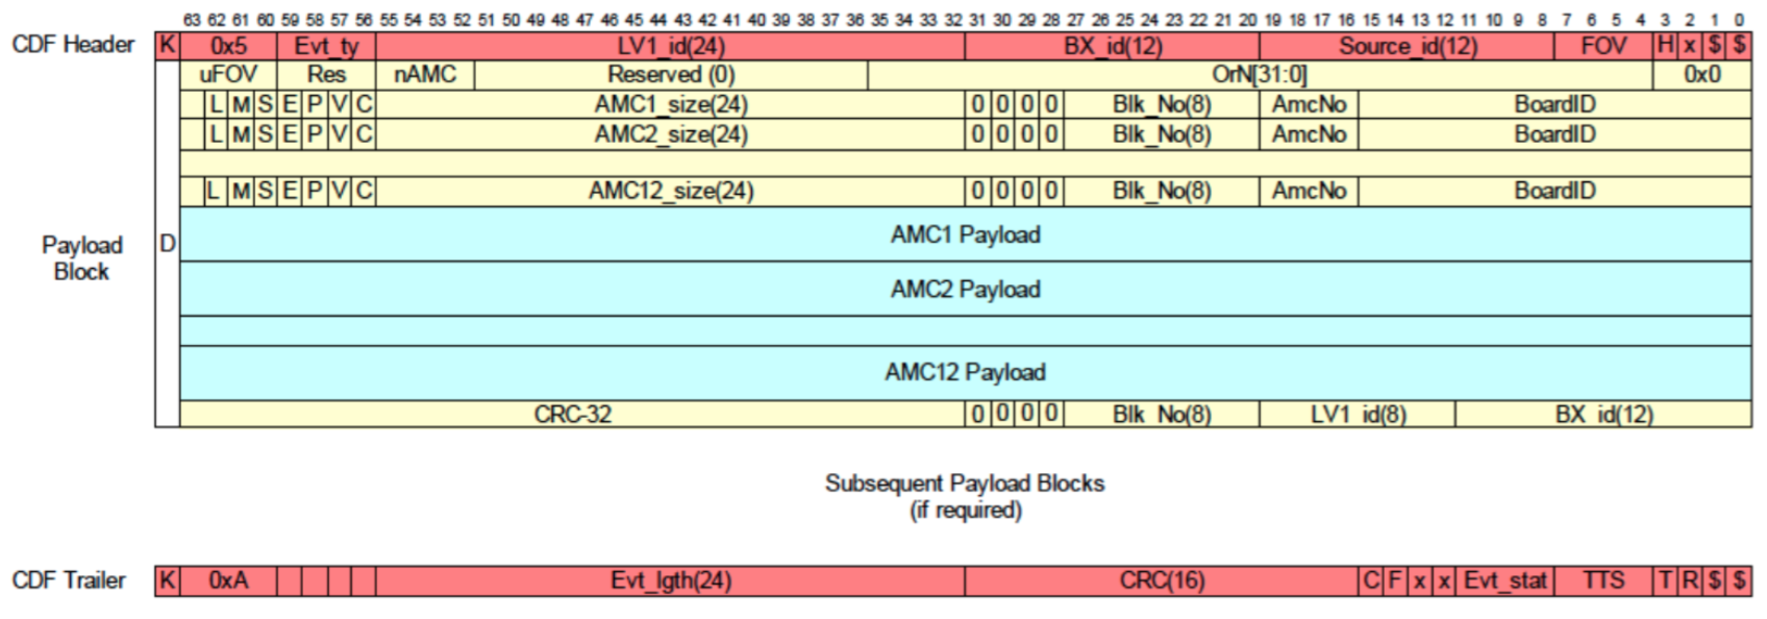
\includegraphics[width=0.85\textwidth]{pics/AMC13ToDAQ.pdf} 
\caption{Data structure for AMC13 to DAQ. The first two 64-bit words are stored in the CA (LA, PA) banks and the last two 64-bit words are stored in the CZ (LZ, PZ) banks.}\label{fig:AMC13ToDAQ}
\end{figure}

\subsubsection*{CA (LA, PA) banks}

This is the bank for the AMC13 to DAQ header information.
The first 64-bit word is the CDF header and the next 64-bit word is the payload header as shown in Fig.~\ref{fig:AMC13ToDAQ}.

\subsubsection*{CZ (LZ, PZ) banks}

This is the bank for the AMC13 to DAQ trailer information.
The first 64-bit word is the last 64-bit word of the payload block and the next 64-bit word is the CDF trailer as shown in Fig.~\ref{fig:AMC13ToDAQ}.


\subsubsection*{CB (LB, PB) banks}

This is the bank for the WFD5 to AMC13 header information as shown in Fig.~\ref{fig:RiderToAMC13}.

\begin{figure}[htbp]
\centering
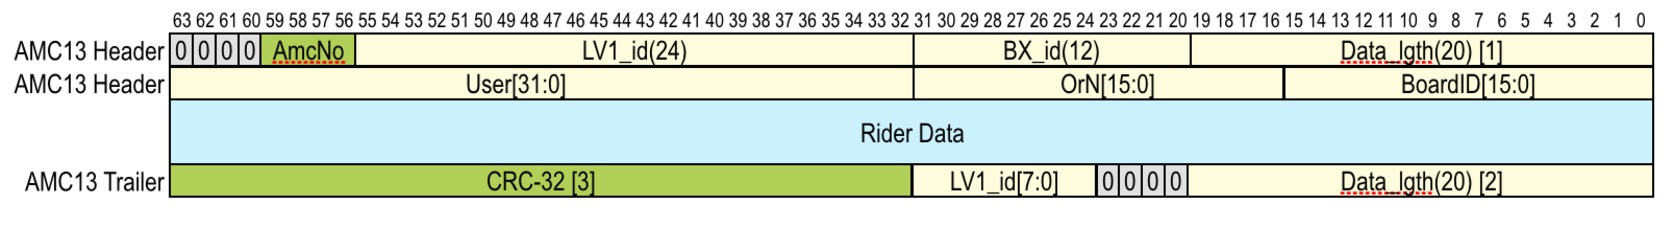
\includegraphics[width=0.85\textwidth]{pics/RiderToAMC13.pdf} 
\caption{Data structure for Rider to AMC13.}\label{fig:RiderToAMC13}
\end{figure}

\subsubsection*{CR (LR, PR) banks}

This is the bank for the full WFD5 payload as shown in Fig.~\ref{fig:RiderData}. Due to the huge data size of raw payload, a pre-scale of about 1000 event is usually being set in the MIDAS ODB.

\begin{figure}[htbp]
\centering
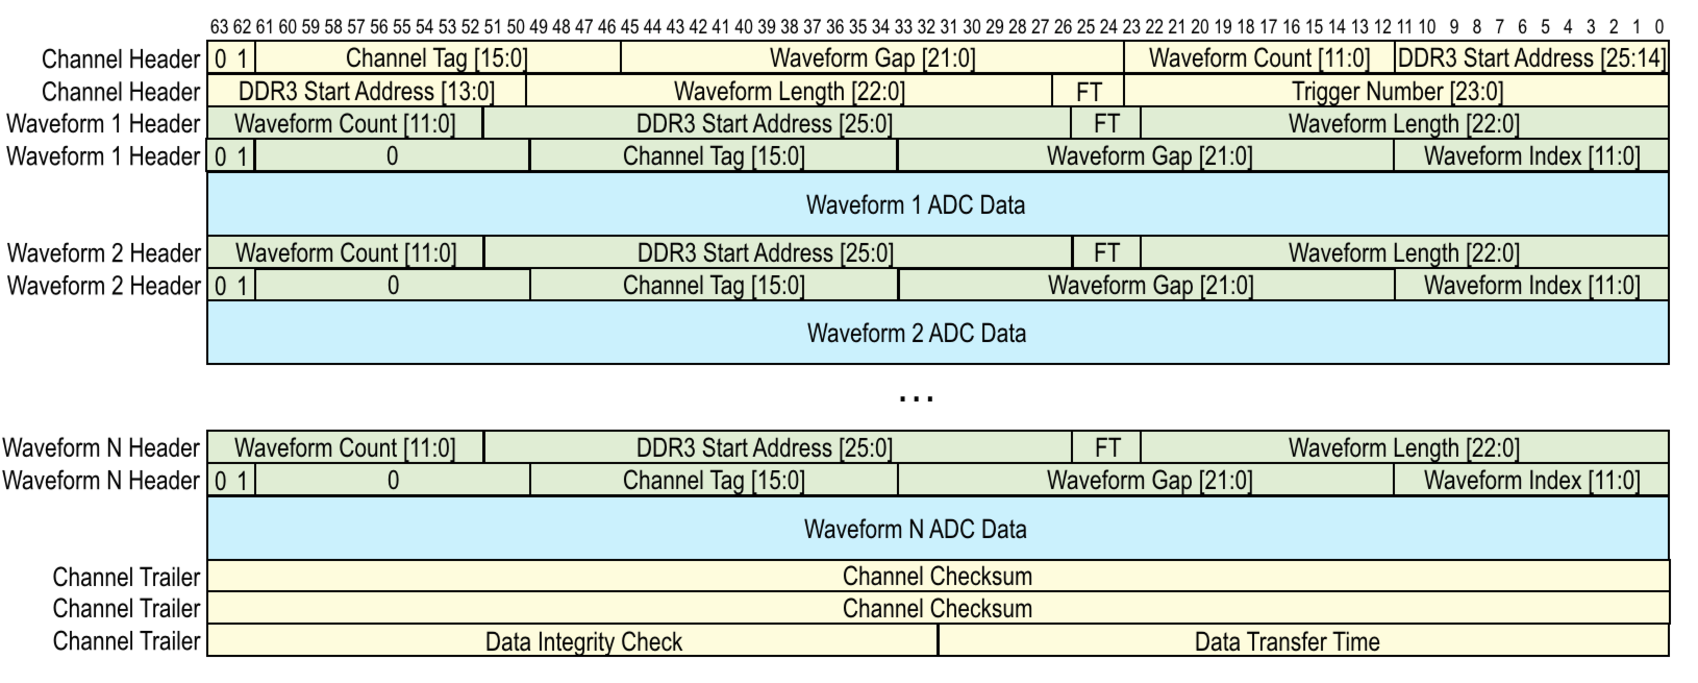
\includegraphics[width=0.85\textwidth]{pics/RiderData.pdf} 
\caption{Data structure for the WFD5 raw payload.}\label{fig:RiderData}
\end{figure}


\subsubsection*{CT (LT, PT) banks}

This is the bank for calorimeter T-method chopped islands. A collection of 54 islands from 54 crystals/segments are extracted per trigger. The detailed structure is shown in Fig.~\ref{fig:CTBankFormat}.

\begin{figure}[htbp]
\centering
\fbox{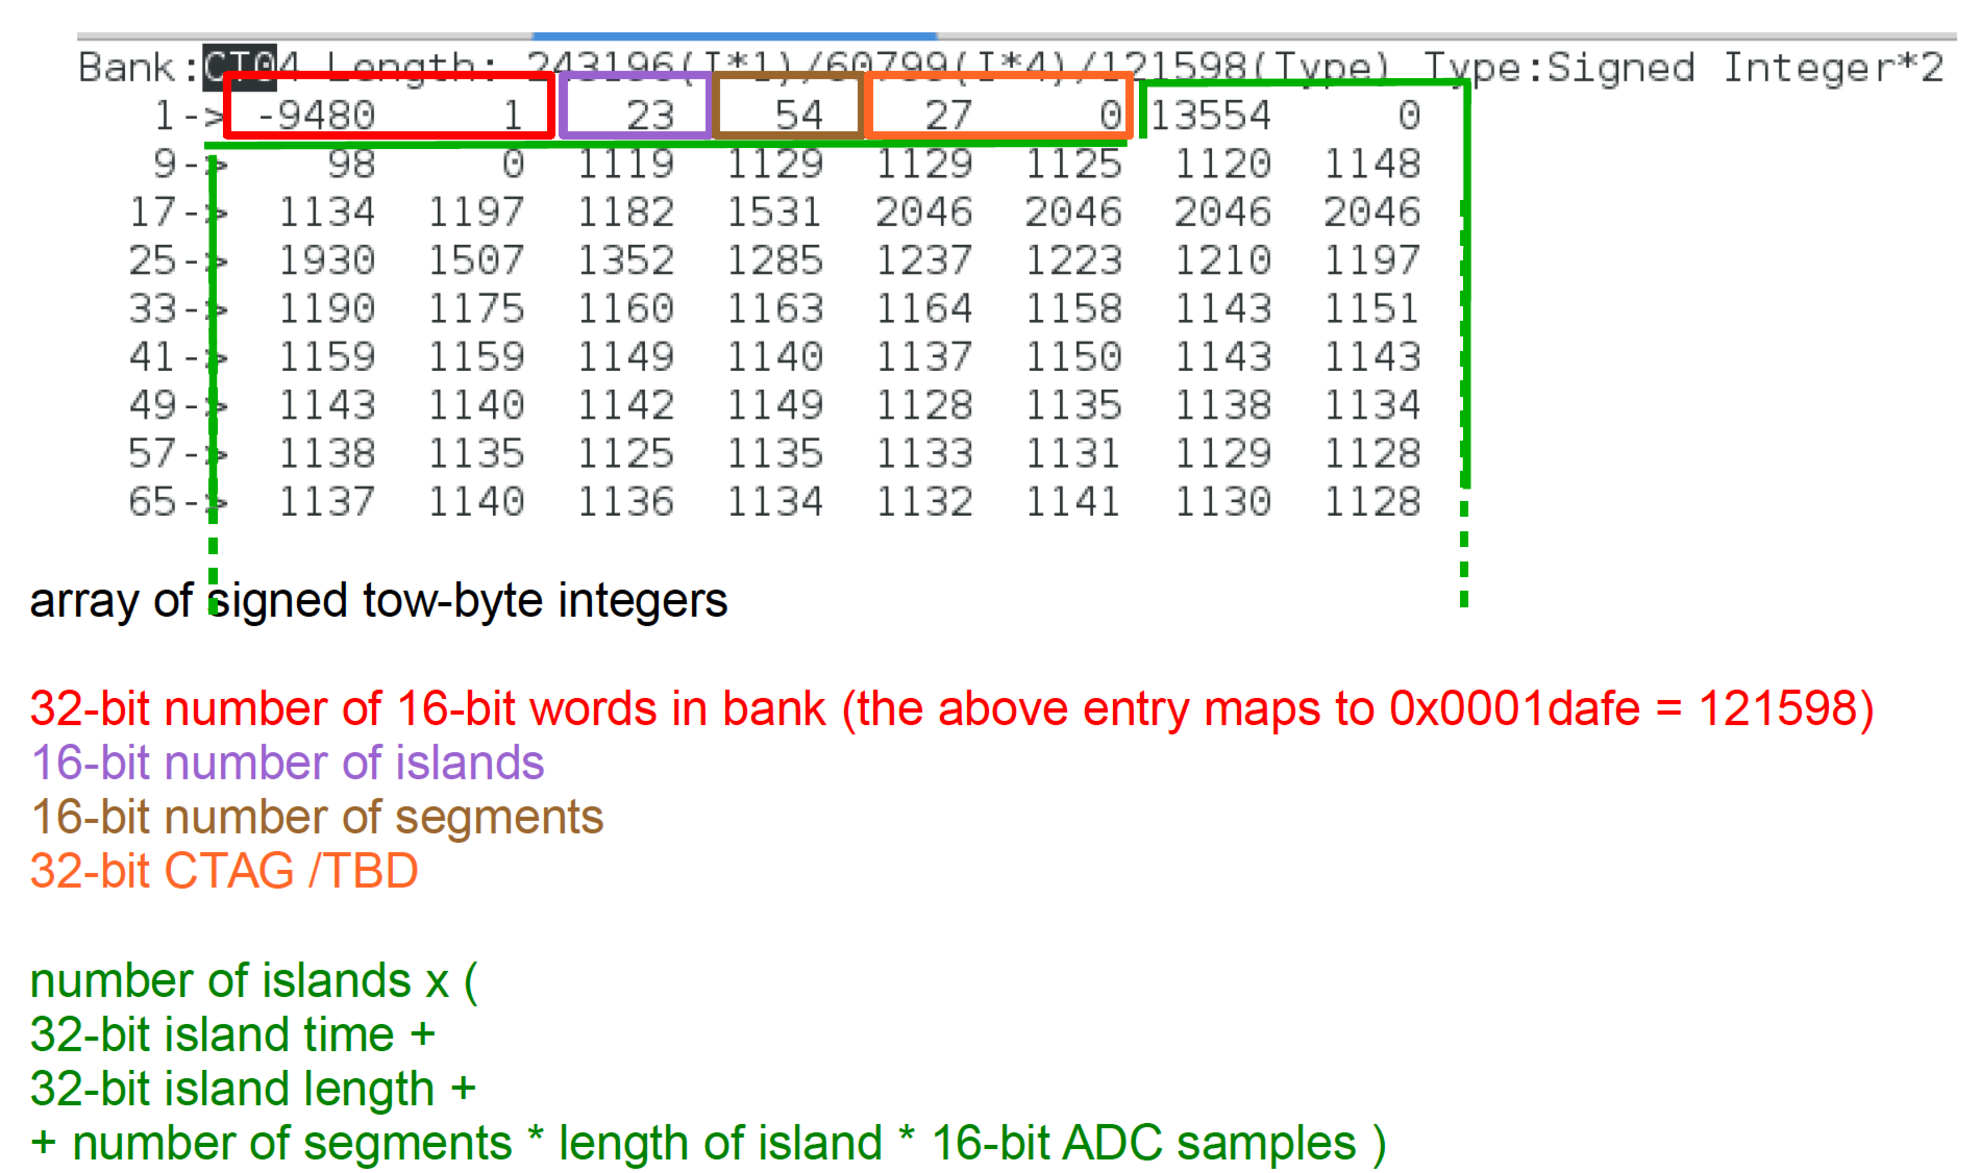
\includegraphics[width=0.75\textwidth]{pics/CTBankFormat.pdf}}
\caption{Data structure for the CT bank (T-method chopped islands).}\label{fig:CTBankFormat}
\end{figure}

\subsubsection*{CH (LH, PH) banks}

This is the bank for calorimeter segment histograms. Histogram from each segment is being summed to itself each fill and is flushed out every N-th event. The detailed structure is shown in Fig.~\ref{fig:CHBankFormat}.

\begin{figure}[htbp]
\centering
\fbox{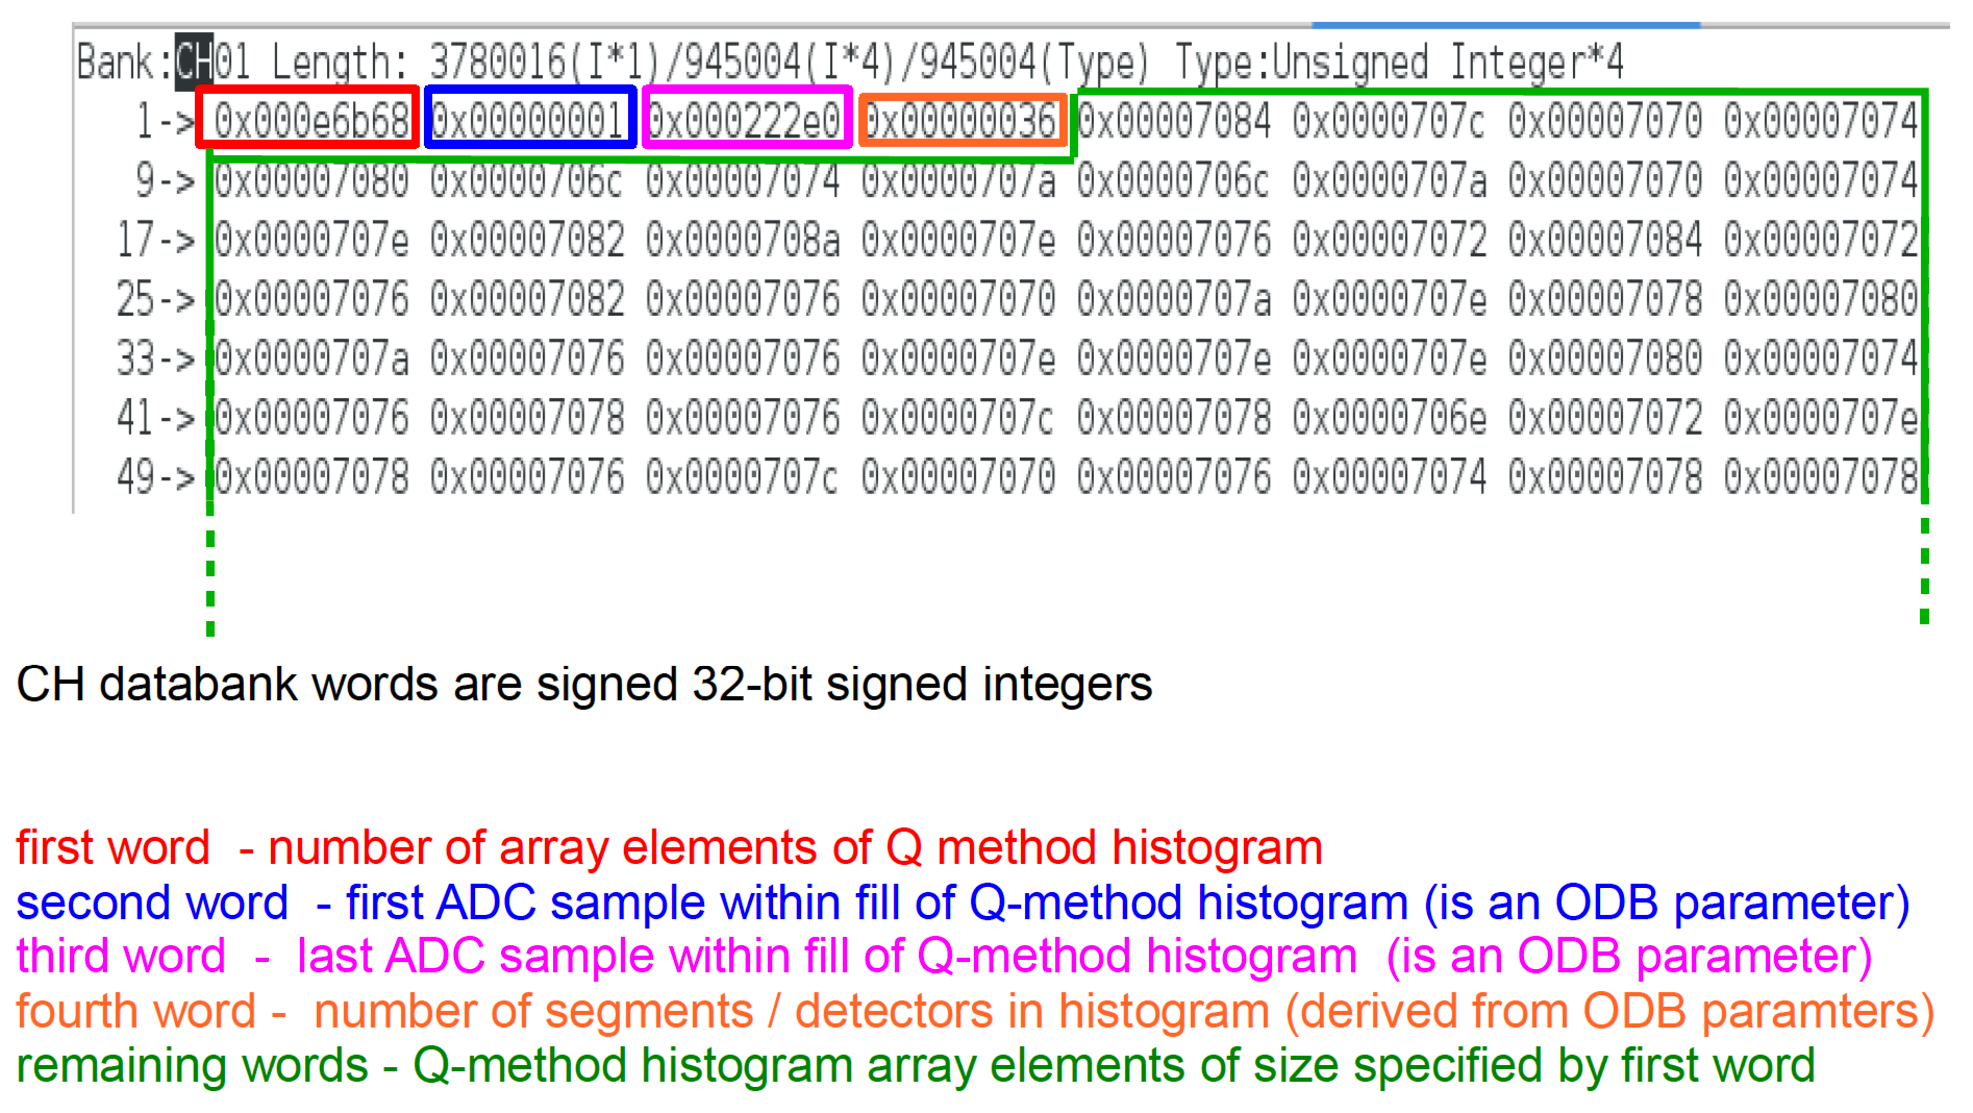
\includegraphics[width=0.75\textwidth]{pics/CHBankFormat.pdf}}
\caption{Data structure for the CH bank (calo segment histograms). In this example, the number of samples $= 512$, initial rebin $= 2$, rebin intervals $=4$ and rebin multiplier $=2$.}\label{fig:CHBankFormat}
\end{figure}

\subsubsection*{CQ (LQ, PQ) banks}

This is the bank for calorimeter sum histograms. Histograms from all segments are summed together and decimated, and then are being flushed out every fill. The detailed structure is shown in Fig.~\ref{fig:CQBankFormat}.

\begin{figure}[htbp]
\centering
\fbox{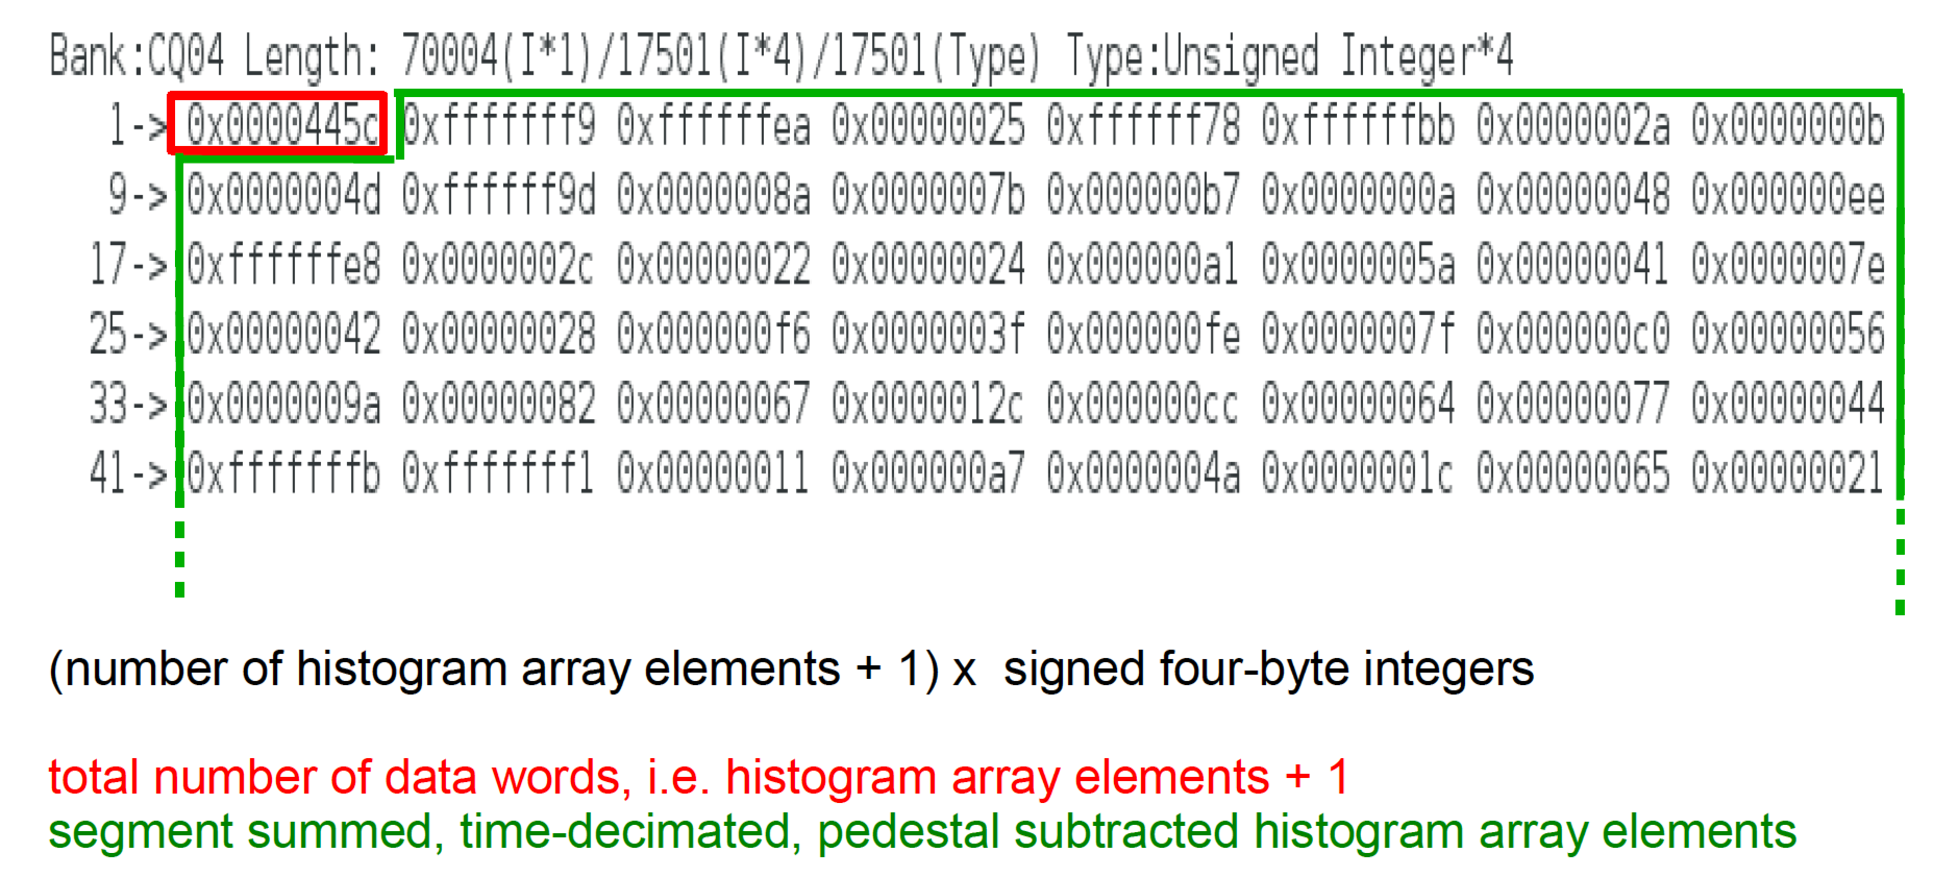
\includegraphics[width=0.75\textwidth]{pics/CQBankFormat.pdf}}
\caption{Data structure for the CQ bank (calo sum histograms).}\label{fig:CQBankFormat}
\end{figure}

\subsubsection*{CP (LP, PP) banks}

This is the bank for calorimeter pedestals. The detailed structure is shown in Fig.~\ref{fig:CPBankFormat}.

\begin{figure}[htbp]
\centering
\fbox{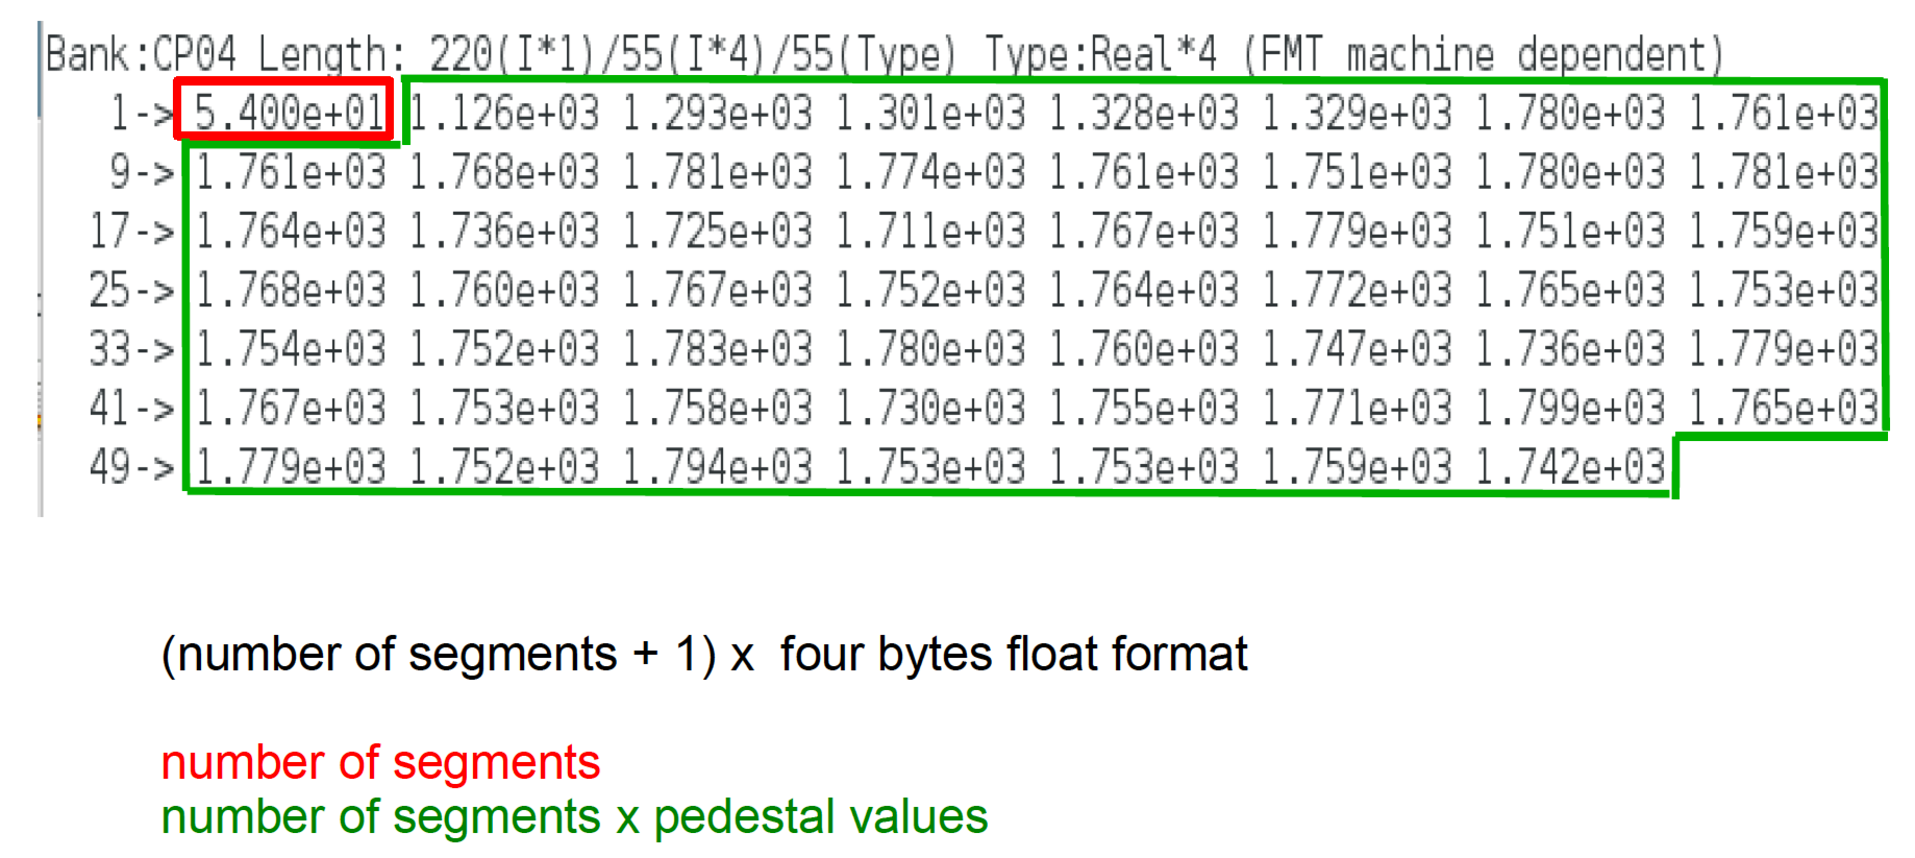
\includegraphics[width=0.75\textwidth]{pics/CPBankFormat.pdf}} 
\caption{Data structure for the CP bank (T-method pedestals).}\label{fig:CPBankFormat}
\end{figure}

\subsubsection*{CC (LC, PC) banks}

This is the bank for the calorimeter DAQ performance related information.
It has information like tcp timing and gpu timing. The detailed structure is shown in Fig.~\ref{fig:CCBankFormat}.

\begin{figure}[htbp]
\centering
\fbox{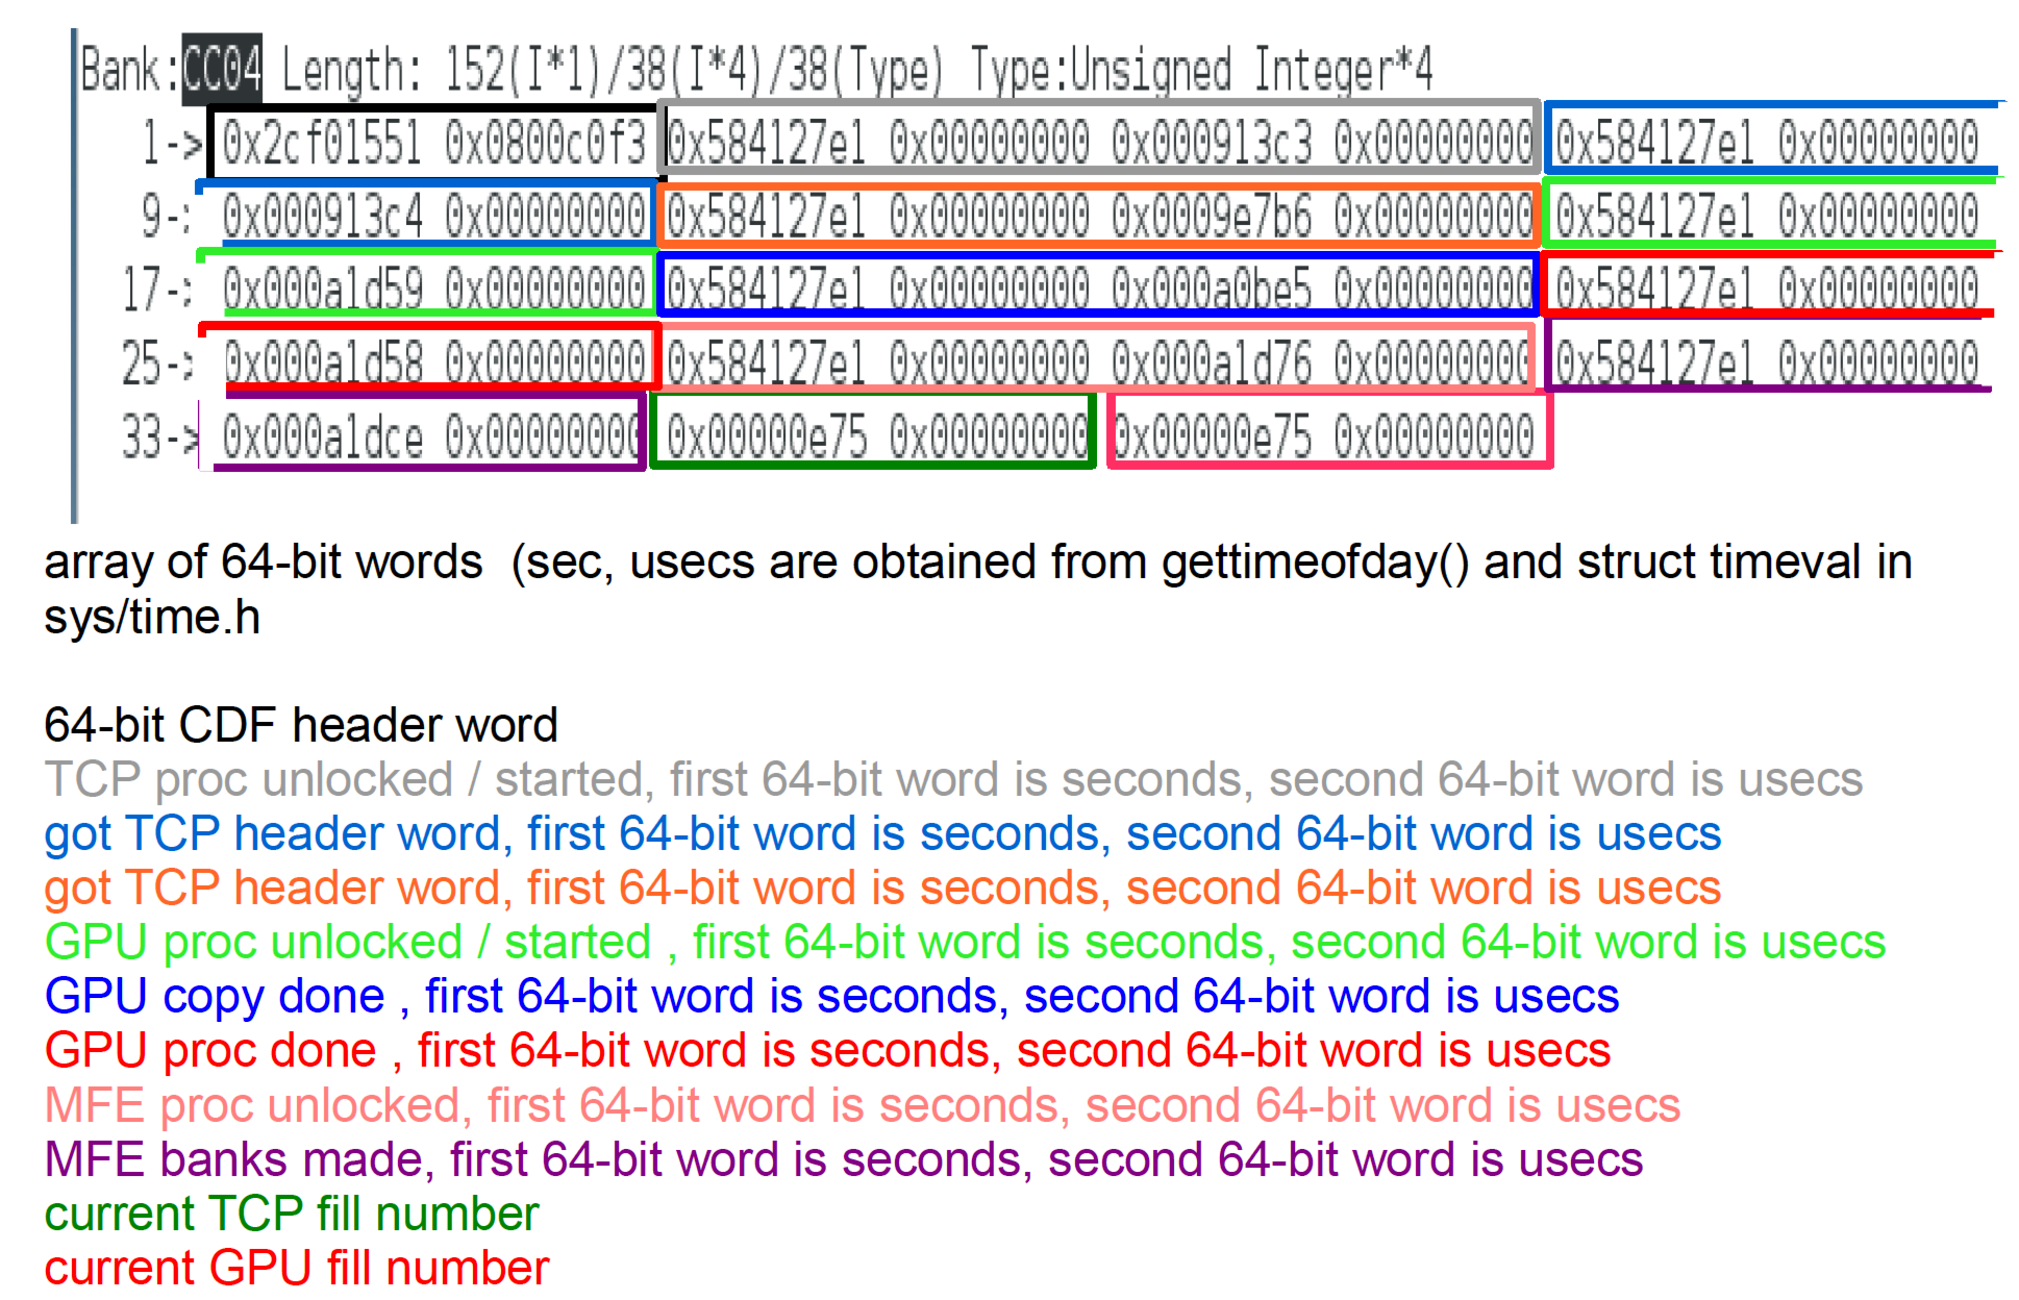
\includegraphics[width=0.75\textwidth]{pics/CCBankFormat.pdf}}
\caption{Data structure for the CC bank (calo performance).}\label{fig:CCBankFormat}
\end{figure}

\subsubsection*{CR (LR, PR) banks, asynchronous}

This is the bank for the WFD5 payload in the asynchronous mode. The detailed structure is shown in Fig.~\ref{fig:AsyncRiderData}.

\begin{figure}[htbp]
\centering
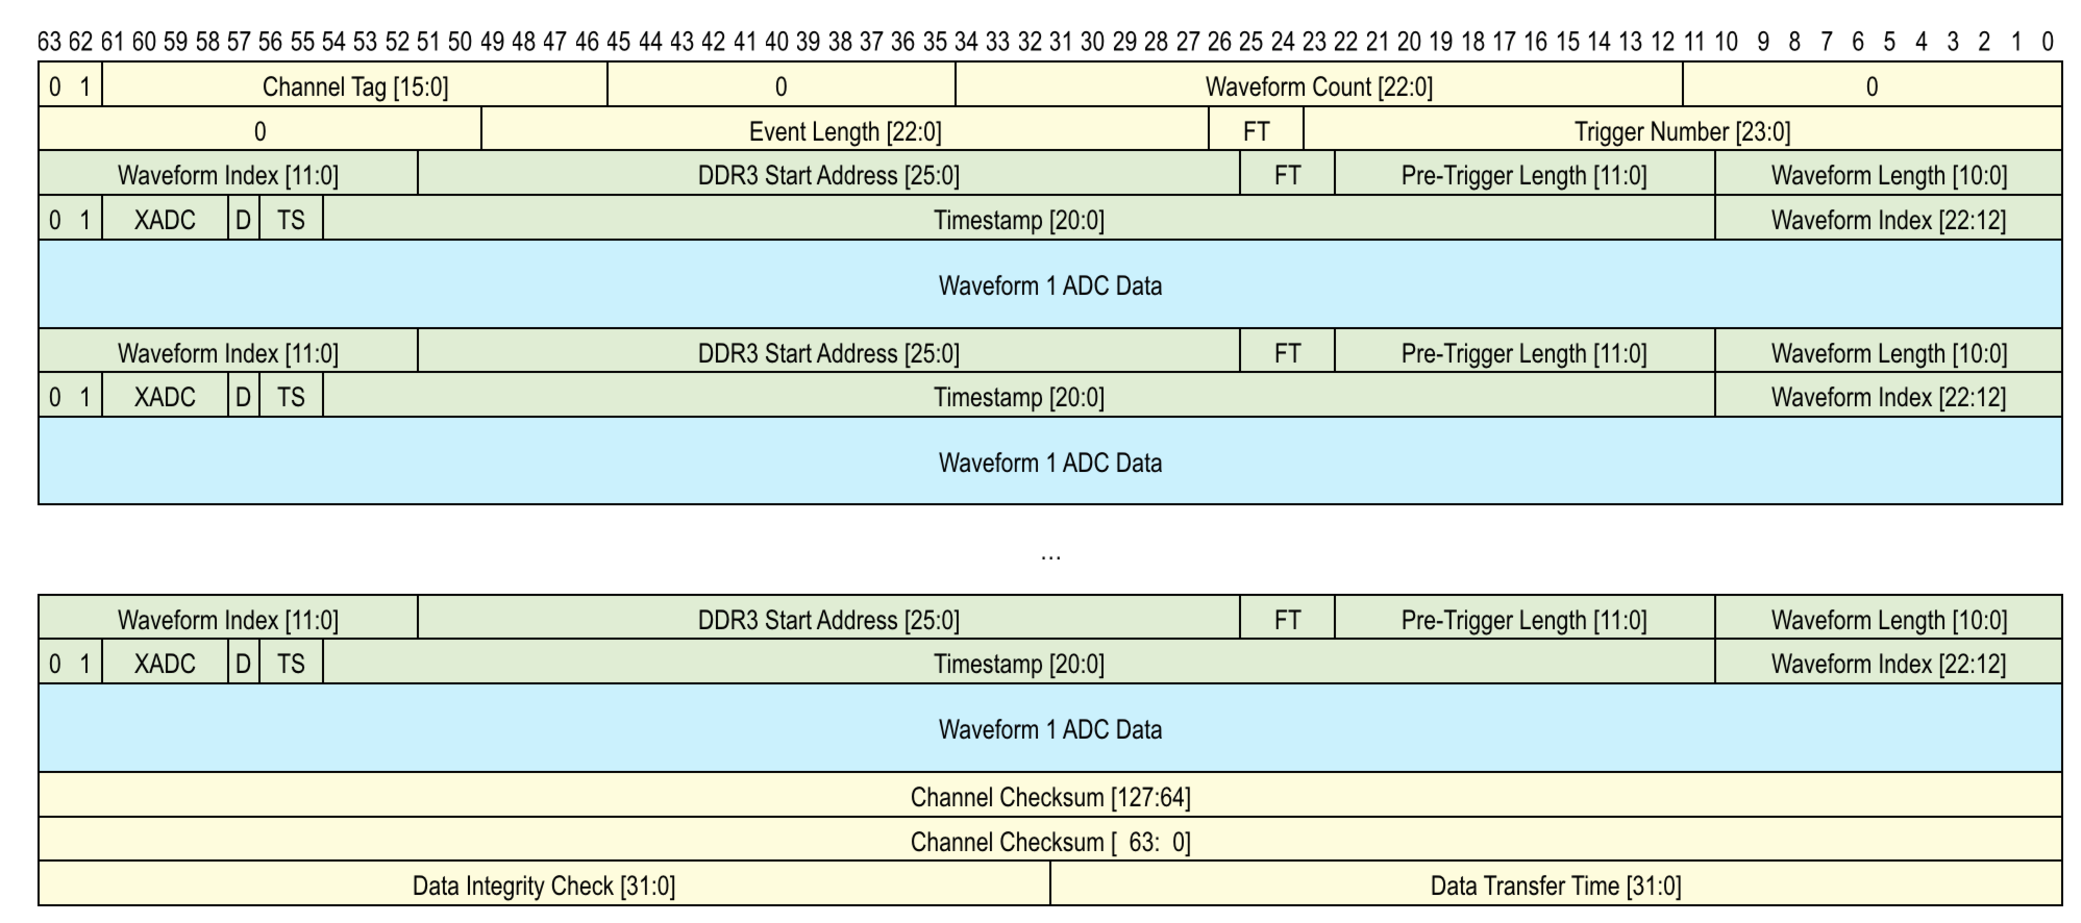
\includegraphics[width=0.9\textwidth]{pics/AsyncRiderData.pdf} 
\caption{Data structure for asynchronous mode for Rider.}\label{fig:AsyncRiderData}
\end{figure}

\subsubsection*{CF banks}

This is the bank for GPU fitted results. The bank starts with an ``unsigned int" that is the number of segments. Then for each of those segments there is a block like this:
an ``unsigned int" which is the number of pulses and then \textit{nPulses} blocks of \textit{pulseFinderResult} struct. The member variables in this struct is shown in Tab.~\ref{tab:cftable}.

\begin{table}[htbp]
\centering
\caption{Format of the struct pulseFinderResult.}
\begin{tabular}{|c|c|c|c|}
\hline
start word index & type & field name & content  \\
\hline
0	& Float\_t & time & fitted time \\
\hline
2	& Float\_t	& phase & fitted phase \\ 
\hline
4	& Float\_t	& energy	& 	fitted energy \\ 
\hline
6	& Float\_t	& pedestal &  fitted pedestal \\ 
\hline
8	& Float\_t	& chi2 &  chi square of the fit \\ 
\hline
10	& Float\_t	& pedestal &  fitted pedestal \\ 
\hline
12	& Int\_t	& peak\_index &  index of the fitted peak\\ 
\hline
14	& Int\_t	& peak\_value &  value of the fitted peak \\ 
\hline
\end{tabular} 
\label{tab:cftable}
\end{table}

\subsection{Auxiliary detector-related banks}

This section will be updated once decision is finalized.

\subsubsection*{KH and KQ banks}
These two banks have the same format as the CH and CQ banks.

\subsubsection*{KT bank}
This bank has the same format as the CT bank.

\subsubsection*{IBMS}
This bank will store all the waveforms from CAEN1742. Actual format to be decided.

\subsection{CCC related banks}

\subsubsection*{TTCA, TTCR, TTCZ banks}

TTCA bank will have the same format as the CA bank in the calorimeter-related data since the uTCA crate has the same data format. TTCZ on the other hand will have the same format as the CZ bank.

There are two types of TTCR banks for the FC7 - encoder and fanout. 
The data format of the encoder and fanout FC7 are shown in Fig.~\ref{fig:EncoderFC7} and Fig.~\ref{fig:FanoutFC7}. respectively.

\begin{figure}[htbp]
\centering
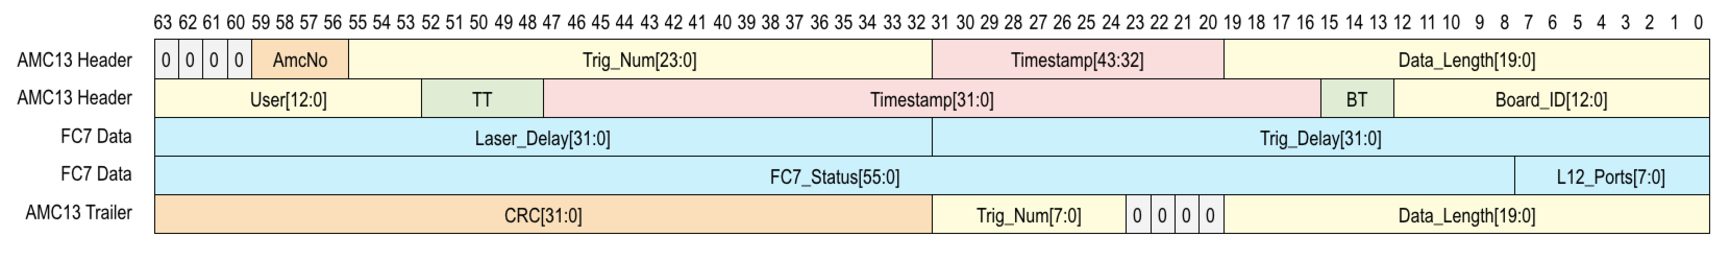
\includegraphics[width=0.9\textwidth]{pics/EncoderFC7.pdf} 
\caption{Data structure for encoder FC7.}\label{fig:EncoderFC7}
\end{figure}

\begin{figure}[htbp]
\centering
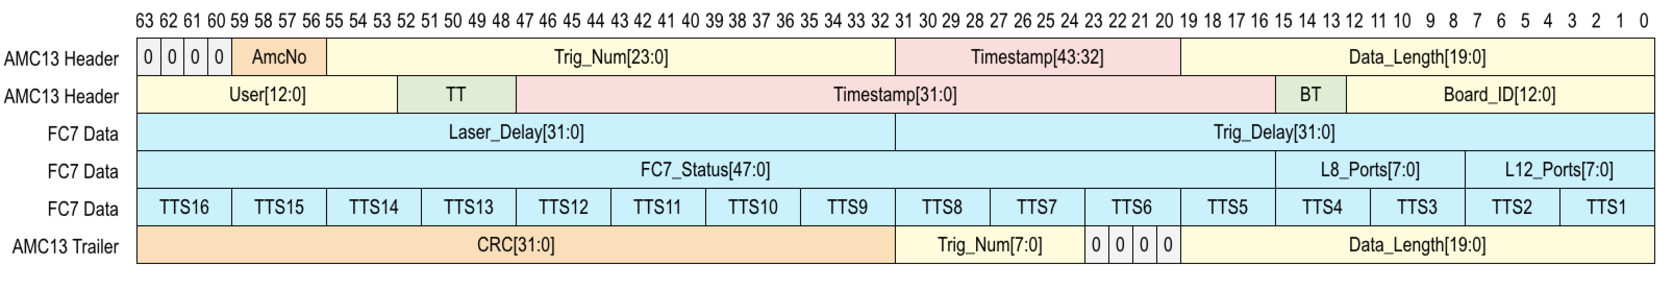
\includegraphics[width=0.9\textwidth]{pics/FanoutFC7.pdf} 
\caption{Data structure for fanout FC7.}\label{fig:FanoutFC7}
\end{figure}


\subsection{Field related banks}

\subsubsection*{FXPR bank}
This is the bank for fixed probes. It consists of a header and NMR waveforms.
Structure of the FXPR bank is summarized in Tab.~\ref{tab:fxprtable} and its macros are summarized in Tab.~\ref{tab:fxprmacro}.

\begin{table}[htbp]
\centering
\caption{MIDAS bank structure for the FXPR bank.}
\begin{tabular}{|c|c|c|c|C{4cm}|c|}
\hline
start word index & type      & array length       & field name & content                                                          & struct name \\
\hline
0                & Double\_t & num\_ch            & sys\_clock & system clock                                                     & \multirow{12}{*}{fixed\_t}                  \\
\cline{1-5}
4*num\_ch        & Double\_t & num\_ch            & gps\_clock & gps clock                                                        &                             \\
\cline{1-5}
8*num\_ch        & Double\_t & num\_ch            & dev\_clock & device clock                                                     &                             \\
\cline{1-5}
12*num\_ch       & Double\_t & num\_ch            & snr        & signal to noise ratio                                            &                             \\
\cline{1-5}
16*num\_ch       & Double\_t & num\_ch            & len        & length of each wave form                                         &                             \\
\cline{1-5}
20*num\_ch       & Double\_t & num\_ch            & freq       & frequency extracted                                              &                             \\
\cline{1-5}
24*num\_ch       & Double\_t & num\_ch            & ferr       & frequency error                                                  &                             \\
\cline{1-5}
28*num\_ch       & Double\_t & num\_ch            & freq\_zc   & frequency extracted, zero crossing                               &                             \\
\cline{1-5}
32*num\_ch       & Double\_t & num\_ch            & ferr\_zc   & frequency error, zero crossing                                   &                             \\
\cline{1-5}
36*num\_ch       & UShort\_t & num\_ch            & health     & health indicator of probes                                       &                             \\
\cline{1-5}
37*num\_ch       & UShort\_t & num\_ch            & method     & frequency extraction method                                      &                             \\
\cline{1-5}
38*num\_ch       & UShort\_t & num\_ch * rec\_len & trace      & NMR waveforms: Waveform\_Ch1 + Waveform\_Ch2 + … + Waveform\_Ch6 &     \\    
\hline
\end{tabular} 
\label{tab:fxprtable}
\end{table}

\begin{table}[htbp]
\centering
\caption{Hard-coded macros in the FXPR bank.}
\begin{tabular}{|c|c|c|}
\hline
Name in the code	& Name in this doc &	Value \\
\hline
NMR\_NUM\_FIXED\_PROBES & num\_ch & 378 \\
\hline
NMR\_FID\_LENGTH\_RECORD & rec\_len & 10000 \\
\hline
\end{tabular} 
\label{tab:fxprmacro}
\end{table}


\subsubsection*{TLNP bank}

This is the bank for Trolley NMR pulses. It consists of a header and NMR waveforms.
Structure of the TLNP bank is summarized in Tab.~\ref{tab:tlnptable} and its macros are summarized in Tab.~\ref{tab:tlnpmacro}.

\begin{table}[htbp]
\centering
\caption{MIDAS bank structure for the TLNP bank.}
\begin{tabular}{|c|c|c|c|C{4cm}|c|}
\hline
start word index &	type	& array length	&field name	&content	& struct name \\
\hline
0	& ULong64\_t & 1 & gps\_clock & Time stamp of the first NMR sample	& \multirow{3}{*}{trolley\_nmr\_t}   \\ 
\cline{1-5}
4	&UShort\_t	& 1 & probe\_index	&probe index	 & \\ 
\cline{1-5}
5	&UShort\_t	&1 & length&	length of the NMR waveform	 & \\ 
\hline
6	&Short\_t & nmr\_len &	trace	&Trolley Probe NMR wavefrom	 & \\ 
\hline
\end{tabular} 
\label{tab:tlnptable}
\end{table}

\begin{table}[htbp]
\centering
\caption{Hard-coded macros in the TLNP bank.}
\begin{tabular}{|c|c|c|}
\hline
Name in the code	& Name in this doc & Value \\
\hline
TRLY\_NMR\_LENGTH	 & nmr\_len & 24000 \\
\hline
\end{tabular} 
\label{tab:tlnpmacro}
\end{table}


\subsubsection*{TLBC bank}
This is the bank for Trolley barcode readers. It consists of a header and barcode waveforms.
Structure of the TLBC bank is summarized in Tab.~\ref{tab:tlbctable} and its macros are summarized in Tab.~\ref{tab:tlbcmacro}.

\begin{table}[htbp]
\centering
\caption{MIDAS bank structure for the TLBC bank.}
\begin{tabular}{|c|c|c|c|C{4cm}|c|}
\hline
start word & index & type & array length & field name	content & struct name \\ 
\hline
0 & ULong64\_t & 1 & gps\_clock & Time stamp of the first barcode sample & \multirow{3}{*}{trolley\_barcode\_t} \\
\cline{1-5}
4 & UShort\_t & 1 & length\_per\_ch & length of the barcode waveform per channel & \\ 
\cline{1-5}	
5 & UShort\_t	& bc\_ch*bc\_len & traces &	Barcode wavefroms: Waveform\_Ch1 + Waveform\_Ch2 + … + Waveform\_Ch6	 &\\
\hline
\end{tabular} 
\label{tab:tlbctable}
\end{table}


\begin{table}[htbp]
\centering
\caption{Hard-coded macros in the TLBC bank.}
\begin{tabular}{|c|c|c|}
\hline
Name in the code	& Name in this doc & Value \\
\hline
TRLY\_BARCODE\_LENGTH	& bc\_len & 3000 \\
\hline
TRLY\_BARCODE\_CHANNELS & bc\_ch & 6 \\
\hline
\end{tabular} 
\label{tab:tlbcmacro}
\end{table}

\subsubsection*{TLMN bank}
This is the bank for Trolley monitors. It consists of information like temperatures, voltages and pressures. Structure of the TLMN bank is summarized in Tab.~\ref{tab:tlmntable} and its macros are summarized in Tab.~\ref{tab:tlmnmacro}.

\begin{table}[htbp]
\centering
\caption{MIDAS bank structure for the TLMN bank.}
\begin{tabular}{|C{2cm}|c|C{1.5cm}|c|C{4cm}|c|}
\hline
start word index & type       & array length & field name               & content                                                & struct name \\
\hline
0                & ULong64\_t & 1            & gps\_clock\_cycle\_start & Time stamp of the measurement cycle                    & \multirow{21}{*}{trolley\_monitor\_t}         \\ 
\cline{1-5}
4                & UInt\_t    & 1            & PMonitorVal              & Pressure Monitor readout value                         &                             \\
\cline{1-5}
6                & Uint\_t    & 1            & PMonitorTemp             & Pressure Monitor temperature                           &                             \\
\cline{1-5}
8                & Uint\_t    & 1            & RFPower1                 & RF Power monitor 1                                     &                             \\
\cline{1-5}
10               & Uint\_t    & 1            & RFPower2                 & RF Power monitor 2                                     &                             \\
\cline{1-5}
12               & Uint\_t    & 1            & NMRCheckSum              & NMR waveform check sum, calculated by trolley inerface &                             \\
\cline{1-5}
14               & Uint\_t    & 1            & FrameCheckSum            & Frame data check sum, calculated by trolley interface  &                             \\
\cline{1-5}
16               & Uint\_t    & 1            & FrameSum                 & Frame data sum calculated by DAQ                       &                             \\
\cline{1-5}
18               & Uint\_t    & 1            & FrameIndex               & Frame index                                            &                             \\
\cline{1-5}
20               & UShort\_t  & 1            & StatusBits               & (Bit 5-7)Reserved                                      &                             \\
\cline{1-5}
21               & UShort\_t  & 1            & TMonitorIn               & Temperature monitor, interia                           &                             \\
\cline{1-5}
22               & UShort\_t  & 1            & TMonitorExt1             & Temperature monitor, exteria 1                         &                             \\
\cline{1-5}
23               & UShort\_t  & 1            & TMonitorExt2             & Temperature monitor, exteria 2                         &                             \\
\cline{1-5}
24               & UShort\_t  & 1            & TMonitorExt3             & Temperature monitor, exteria 3                         &                             \\
\cline{1-5}
25               & UShort\_t  & 1            & V1Min                    & Voltage Monitor 1, mininum                             &                             \\
\cline{1-5}
26               & UShort\_t  & 1            & V1Max                    & Voltage Monitor 1, maximum                             &                             \\
\cline{1-5}
27               & UShort\_t  & 1            & V2Min                    & Voltage Monitor 2, mininum                             &                             \\
\cline{1-5}
28               & UShort\_t  & 1            & V2Max                    & Voltage Monitor 2, maximum                             &                             \\
\cline{1-5}
29               & UShort\_t  & 1            & length\_per\_ch          & waveform length per channel for the voltage monitors   &                             \\
\cline{1-5}
30               & UShort\_t  & mn\_len      & trace\_VMonitor1         & waveform of voltage monitor 1                          &                             \\
\cline{1-5}
30+mn\_len       & UShort\_t  & mn\_len      & trace\_VMonitor2         & waveform of voltage monitor 2                         &     \\
\hline
\end{tabular} 
\label{tab:tlmntable}
\end{table}


\begin{table}[htbp]
\centering
\caption{Hard-coded macros in the TLMN bank.}
\begin{tabular}{|c|c|c|}
\hline
Name in the code	& Name in this doc & Value \\
\hline
TRLY\_MONITOR\_LENGTH & mn\_len & 3000 \\
\hline
\end{tabular} 
\label{tab:tlmnmacro}
\end{table}


\subsubsection*{GALI bank}

This is the bank for trolley and garage data. It has information like the trolley positions and velocities. Structure of the GALI bank is summarized in Tab.~\ref{tab:galitable1} and \ref{tab:galitable2}, and its macros are summarized in Tab.~\ref{tab:galimacro}.


\begin{table}[htbp]
\centering
\caption{MIDAS bank structure for the GALI bank.}
\begin{tabular}{|c|c|c|c|c|c|}
\hline
start word index & type           & array length & field name & content  & struct name \\
\hline
0                & galil\_data\_t & group\_size  & -          & Array of structs: galil\_data\_t & galil\_data\_t              \\
\hline
\end{tabular}
\label{tab:galitable1}
\end{table}

\begin{table}[htbp]
\centering
\caption{Format of the struct galil\_data\_t.}
\begin{tabular}{|c|c|c|c|C{5cm}|}
\hline
start word index & type & array length & field name	 & content \\
\hline
0  & ULong64\_t & 1 & TimeStamp  & time stamp of the readout                         \\
\hline
4  & Int\_t     & 2 & Tensions   & Tensions of the fishing line and the signal cable \\
\hline
8  & Int\_t     & 3 & Positions  & Positions: Motor 1, Motor 2 and Garage            \\
\hline
14 & Int\_t     & 3 & Velocities & Velocities: Motor 1, Motor 2 and Garage           \\
\hline
20 & Int\_t     & 3 & OutputVs   & Output voltages: Motor 1, Motor 2 and Garage  \\
\hline
\end{tabular}
\label{tab:galitable2}
\end{table}

\begin{table}[htbp]
\centering
\caption{Hard-coded macros in the GALI bank.}
\begin{tabular}{|c|c|c|}
\hline
Name in the code	& Name in this doc & Value \\
\hline
GALILREADGROUPSIZE & group\_size & 50 \\
\hline
\end{tabular} 
\label{tab:galimacro}
\end{table}

\subsubsection*{ABPR bank}

This is the bank for absolute probe data. Both spherical probe and plunging probe are using the same bank. It has information like the header and NMR waveforms. Structure of the ABPR bank is summarized in Tab.~\ref{tab:abprtable}.

\begin{table}[htbp]
\centering
\caption{MIDAS bank structure for the ABPR bank.}
\begin{tabular}{|c|c|c|c|C{3cm}|c|}
\hline
start word index & type       & array length & field name        & content                      & struct name \\
\hline
0                & ULong64\_t & 1            & time\_stamp       & Time stamp of the NMR sample & \multirow{5}{*}{absolute\_nmr\_info\_t}      \\
\cline{1-5}
4                & Uint\_t    & 1            & length            & probe index                  &                             \\
\cline{1-5}
6                & Uint\_t    & 4            & position          & length of the NMR waveform   &                             \\
\cline{1-5}
14               & UShort\_t  & 1            & flay\_run\_number & Trolley Probe NMR wavefrom   &                             \\
\cline{1-5}
15               & UShort\_t  & 1            & probe\_index      &                              &                             \\
\hline
16               & UShort\_t  & length       & -                 & NMR waveform\footnotemark &    \\
\hline
\end{tabular}
\label{tab:abprtable}
\end{table}
\footnotetext{Note: the length of the NMR waveform is not fixed from event to event. For each event, its length is determined by the "length" field of the "absolute\_nmr\_info\_t" struct in the header section.}

\subsubsection*{FLUX bank}

This is the bank for the fluxgate. It has information like the fluxgate waveforms. Structure of the FLUX bank is summarized in Tab.~\ref{tab:fluxtable} and its macros are summarized in Tab.~\ref{tab:fluxmacro}.

\begin{table}[htbp]
\centering
\caption{MIDAS bank structure for the FLUX bank.}
\begin{tabular}{|c|c|c|c|C{3cm}|c|}
\hline
start word index & type    & array length        & field name & content                                                                  & struct name \\
\hline
0                & float64 & num\_ch*period*rate & -          & Flux gate wave forms for all channels: Waveform\_ch1 + Waveform\_ch2 + … &     \\
\hline        
\end{tabular}
\label{tab:fluxtable}
\end{table}

\begin{table}[htbp]
\centering
\caption{Hard-coded macros in the FLUX bank.}
\begin{tabular}{|c|c|c|}
\hline
Name in the code    & Name in this doc & Value \\
\hline
FLUX\_NUM\_CHANNELS & num\_ch          & 9     \\
\hline
FLUX\_TRACE\_PERIOD & period           & 60    \\
\hline
FLUX\_RATE          & rate             & 8000 \\
\hline
\end{tabular} 
\label{tab:fluxmacro}
\end{table}

\subsubsection*{SFCL bank}

This is the bank for the surface coil. It has the information like current readouts from the surface coils. Structure of the SFCL bank is summarized in Tab.~\ref{tab:sfcltable} and its macros are summarized in Tab.~\ref{tab:sfclmacro}.

\begin{table}[htbp]
\centering
\caption{MIDAS bank structure for the SFCL bank.}
\begin{tabular}{|c|c|c|c|C{3cm}|c|}
\hline
start word index & type      & array length & field name & content               & struct name \\
\hline
0                & Double\_t & num\_coil    & sys\_clock & system clock          & \multirow{4}{*}{surface\_coil\_t}     \\
\cline{1-5}
4*num\_coil      & Double\_t & num\_coil    & gps\_clock & gps clock             &                             \\
\cline{1-5}
8*num\_coil      & Double\_t & num\_coil    & top\_board & top board currents    &                             \\
\cline{1-5}
12*num\_coil     & Double\_t & num\_coil    & bot\_board & bottom board currents & \\
\hline        
\end{tabular}
\label{tab:sfcltable}
\end{table}


\begin{table}[htbp]
\centering
\caption{Hard-coded macros in the SFCL bank.}
\begin{tabular}{|c|c|c|}
\hline
Name in the code    & Name in this doc & Value \\
\hline
SC\_NUM\_COILS &  num\_coil & 100 \\
\hline
\end{tabular} 
\label{tab:sfclmacro}
\end{table}
%%%%%%%%%%%%%%%%%%%

\newpage
\section{Parsers for MIDAS bank data}
Muon g-2 offline analysis framework relies on parsers in the gm2parser namespace hosted under repository gm2unpackers to decode the data. To checkout the codes, 

\begin{Verbatim}[frame=single]
git clone ssh://p-gm2dqm@cdcvs.fnal.gov/cvs/projects/gm2unpackers
\end{Verbatim}
%
Alternatively, you can also use 
\begin{Verbatim}[frame=single]
mrb g gm2dqm
\end{Verbatim}
in our g-2 environment.
%
These parsers are written in C++ and are being used in the \textit{art} producer modules. They can also be used in your standalone C++ codes, if you wish to. The parsers are located at
%
\begin{Verbatim}[frame=single]
gm2unpackers/calo/parsers
\end{Verbatim}
at the moment for both calorimeter and CCC related information. This section will be updated accordingly once they are reorganized.


\section{Cheat sheet for data unpacking}\label{sec:cheatsheet}

A complete list of midas bank to unpacker to data product is summarized in Tab.~\ref{tab:cheatsheet}. 

\begin{table}[htbp]
\centering
\caption{Midas bank-Data unpacker-Data product relationship table. This is the mapping as of Jan 10, 2017 and will be updated accordingly once the restructuring of the data unpacking is completed.}
\begin{tabular}{|c|c|c|}
\hline
Midas bank & Data unpacker (\textit{art} producer module) & Data product (\textit{struct}) \\
\hline
\multirow{3}{*}{CR} & \multirow{3}{*}{RawUnpacker} & gm2calo::RiderArtRecord \\
& & gm2calo::AMCHeader \\
& & gm2calo::RiderChannelHeader \\
\hline
\multirow{3}{*}{LR, PR} & \multirow{3}{*}{RawUnpacker} & gm2calo::IslandArtRecord \\
& & gm2calo::AMCHeader \\
& & gm2calo::RiderChannelHeader \\
\hline
\multirow{3}{*}{CR25} & \multirow{3}{*}{LaserRawUnpacker} & gm2calo::RiderArtRecord \\
& & gm2calo::AMCHeader \\
& & gm2calo::RiderChannelHeader \\
\hline
CT & IslandUnpacker & gm2calo::IslandArtRecord \\
\hline
\multirow{2}{*}{CB} & \multirow{2}{*}{HeaderUnpacker} & gm2calo::AMCHeader \\
\cline{3-3}
& & gm2calo::CDFHeader \\
\hline
CH & CHUnpacker & gm2calo::QHistArtRecord \\
\hline
TTCR & FC7Unpacker & gm2calo::FC7Header \\
\hline
CF & GpuFitResultUnpacker & gm2calo::FitResultArtRecord \\
\hline
\end{tabular} 
\label{tab:cheatsheet}
\end{table}


\begin{thebibliography}{9}
\bibitem{Midas}
TRIUMF MIDAS homepage, accessed Jan 5, 2017. 
\url{https://midas.triumf.ca/MidasWiki/index.php/Main_Page}

\end{thebibliography}

\end{document}
